% !TEX root = ../main.tex
\ulfgchapter{8}{Closing the Domain Gap}{chp:domaingap}

\section{Introduction}

Chapter~\ref{chp:realdata} ended on a negative result and a measurement. The negative result is
that the synthetic margin did not survive transfer: frozen on real data, the learned detector and
CA-CFAR became statistically indistinguishable in exact-support recall while the learned arm
emitted roughly twice the output. The measurement is the domain audit, which found the simulator
and the real sensor to differ in background smoothness, spread, ridge structure and range
behaviour by margins far larger than any tuning constant in the project.

Those two things together pose an obvious question, and this chapter answers it in two steps.

\begin{description}
\itemsep3pt
\item[Stage 4 --- target-domain-informed synthetic training.] If the synthetic \emph{training}
domain is made statistically closer to the real one, does transfer improve --- \emph{without any
real radar frame entering neural optimisation}? This isolates the training distribution as the
variable.
\item[Stage 5 --- real-domain fine-tuning.] If real supervision is finally permitted, can the same
$\TinyParams$-parameter network exceed CA-CFAR on real sequences at a comparable output burden?
This is the first and only point in the thesis where a real radar frame reaches a gradient.
\end{description}

\textbf{What these two experiments are, stated plainly.} Neither is a fresh zero-shot external
validation, and neither is presented as one. Chapter~\ref{chp:realdata}'s evaluation was the single
pre-registered read of the CARRADA test split; everything here comes afterwards and is reported as
a follow-up. Appendix~\ref{app:prereg} records the chronology.

\section{Stage 4: domain-informed synthetic training}
\label{sec:stage4}

\subsection{Motivation and what is being isolated}

The domain audit of Section~\ref{sec:r0} measured differences, not causes. Stage 4 turns
one of those measurements into an intervention: the synthetic background is rebuilt so that its
\emph{measured} statistics move toward the real ones, and everything else is held fixed. If transfer
improves, the training distribution mattered. If it does not, the loss of the margin lies elsewhere.

\subsection{Calibration from the training split only}

The generator's parameters were derived from the \textbf{18 official CARRADA training sequences and
nothing else}. The validation split was not used, and the test split was not opened by any code that
influenced the design. Three background properties were changed, all of them set from train-derived
measurements:

\begin{itemize}
\itemsep2pt
\item \textbf{Multi-look-like smoothness.} The original chain produces a single-look background: its
measured spread is \SI{5.569}{\decibel} against the closed-form single-look value of
\SI{5.570}{\decibel}. The real background behaves like an incoherent average of roughly seven to
eight looks. Frames are therefore formed as a power average of several independent background
realisations sharing one deterministic target field.
\item \textbf{Range-dependent mean background.} The measured train range profile, unit-mean in
power, is applied to the background alone --- never to the targets, whose amplitudes come from the
frozen radar equation.
\item \textbf{A narrow, persistent zero-Doppler ridge.} Strong, about one bin wide at half power,
and present in essentially every frame rather than in the minority of frames the original strata
produced.
\end{itemize}

The target model, the point spread function, the range and Doppler windows, the labels, the target
placement, the SNR sampling and the dataset sizes are untouched. Only the background changed.

\subsection{What could not be matched, and why}

This is a \textbf{partial domain-gap reduction}, not a reproduction of CARRADA. Two mismatches
survive deliberately, and both trace to one frozen constraint.

The lag-1 Doppler correlation of the real background is far lower than the simulator's. That
correlation is set by the slow-time window, and the same window defines the target point spread
function, the measured mainlobe width and hence the guard geometry that makes the CFAR comparison
fair. Changing it would change the detector contract established in Chapter~\ref{chp:detectors}, so
it was left alone and declared. The same constraint widens the synthetic ridge's skirt relative to
the real one, whose fall-off is sharper than any window of this family permits. Both residuals were
recorded before any model was trained.

\subsection{Result on the CARRADA test split}

Eight seeds were trained on the revised synthetic domain under the frozen training contract ---
same architecture, optimiser, learning rate, batch size, epoch count, positive weighting and flat
$3\times3$ label --- and thresholds were derived from the new synthetic validation split alone.

\begin{table}[H]
\centering
\caption{Stage 4 on the \textbf{CARRADA test split}: exact dense-mask object recall over
\CiTestObjects{} eligible objects, and output burden. The difference is sequence-balanced over the
\CiTestNseq{} test sequences.}
\label{tab:stage4}
\begin{tabular}{@{}lcc@{}}
\toprule
\textbf{Arm} & \textbf{Exact recall} & \textbf{Unmatched det./frame} \\
\midrule
Original synthetic TinyCNN            & \CiTestOrig & \CiTestBurdenOrig \\
\textbf{CARRADA-informed TinyCNN}     & \textbf{\CiTestNew} & \textbf{\CiTestBurdenNew} \\
CA-CFAR                               & \CiTestCFAR & \CiTestBurdenCFAR \\
\midrule
\multicolumn{3}{@{}l@{}}{Informed $-$ original: \CiTestDelta{}, 95\,\% CI
[\CiTestCIlo{}, \CiTestCIhi{}], positive on \CiTestSeqAhead{} of \CiTestNseq{} sequences} \\
\bottomrule
\end{tabular}
\end{table}

Recall rose by \CiTestDelta{}, with an interval clear of zero and the same sign on every test
sequence. The pre-specified range question was answered too: in the nearest block, where
Chapter~\ref{chp:realdata} measured the largest deficit, recall moved from \CiTestNearOrig{} to
\CiTestNearNew{} against CA-CFAR's \CiTestNearCFAR{} --- the deficit closed.

\subsection{The cost, which is the other half of the result}

\begin{quote}
\textbf{The recall gain was bought with output density.} Unmatched detections rose from
\CiTestBurdenOrig{} to \CiTestBurdenNew{} per frame, a factor of \CiTestBurdenRatio{}, against
CA-CFAR's \CiTestBurdenCFAR{}.
\end{quote}

A detector that fires more often recovers more objects, so a burden-matched diagnostic was run to
ask whether anything survived once output was equalised. Two things did, and they point in opposite
directions. The informed arm beats the original arm at \emph{equal} output, so the gain is not
merely density. But CA-CFAR leads \emph{both} learned arms at every matched burden level.

\textbf{Supported conclusion.} Reducing the measured synthetic-to-real background mismatch
substantially changed transfer behaviour and recovered much of the learned detector's real-data
recall, without any real frame entering neural optimisation. It did \textbf{not} establish
superiority over CA-CFAR once detector output burden is controlled.

\subsection{What this stage can and cannot attribute}

Several background properties changed together. The experiment supports a causal statement about
the \emph{combined} intervention --- changing the synthetic training domain toward the measured
target statistics changed transfer performance --- and nothing narrower. It does not establish that
the smoothness, the ridge or the range profile was individually responsible. Separating them would
need one ablation per property, which the General Conclusion lists as future work and this thesis
does not claim to have run.

\section{Stage 5: real-domain fine-tuning}
\label{sec:stage5}

\subsection{Motivation}

Stage 4 recovered recall and left an efficiency problem. Stage 5 asks the question the whole thesis
has been circling: with real supervision finally permitted, can the same small network exceed the
classical baseline at a comparable output burden?

\subsection{Protocol}

Fine-tuning starts from each of the eight Stage-4 checkpoints, preserving seed identity, and uses
\textbf{CARRADA training sequences only}. The 18 training sequences were divided at
\textbf{sequence level} into \FtFitSeq{} for fitting and \FtDevSeq{} for internal development;
frames from one recording never straddle the two sides, because consecutive frames of a sequence are
near-duplicates and a frame-level split would leak one into the other almost perfectly.

\textbf{The supervision changes here, and that is the point.} The synthetic arms were trained on
flat $3\times3$ blocks around point targets. Fine-tuning uses the \textbf{provided dense
segmentation masks}, restricted to the detector-valid interior, with annotation-empty frames kept as
genuine all-background examples. Nothing is invented: no centroids, no brightest cells, no
bounding-box centres. This is therefore real-domain \emph{adaptation}, not a continuation of the
original point-target task.

All layers train, including the normalisation statistics --- a $\TinyParams$-parameter network has
no sub-network worth freezing. The architecture is untouched. The configuration is deliberately
small: \num{1e-4} learning rate, ten epochs at most, early stopping on internal-development loss,
positive weight \FtPosWeight{} fixed by a rule declared before the class balance was measured.

\textbf{The operating point was fixed before the evaluation split was opened.} CARRADA cannot
support a false-alarm measurement, so the threshold cannot be set by a measured $\Pfa$ as it is on
synthetic data. Instead, CA-CFAR was run on the three internal-development sequences and its output
burden measured (\FtCaDevBurden{} unmatched detections per frame); each seed's threshold is the one
maximising exact recall on those sequences subject to not exceeding that burden. This produces a
burden-matched operating point using training data alone.

\subsection{Result on previously unscored validation sequences}

The official CARRADA validation split had never been scored by any detector, nor used for any model
or threshold decision. It was read once, after the configuration above was frozen and hashed.

\begin{table}[H]
\centering
\caption{Stage 5 on the \textbf{CARRADA validation split}: \FtValFrames{} frames,
\FtValObjects{} eligible objects. This is a \emph{different} split from Table~\ref{tab:stage4};
values in the two tables are not paired measurements.}
\label{tab:stage5}
\begin{tabular}{@{}lcc@{}}
\toprule
\textbf{Arm} & \textbf{Exact recall} & \textbf{Unmatched det./frame} \\
\midrule
Original synthetic TinyCNN        & \FtValOrig & \FtValBurdenOrig \\
CARRADA-informed TinyCNN          & \FtValCi   & \FtValBurdenCi \\
\textbf{Real-fine-tuned TinyCNN}  & \textbf{\FtValFt} & \textbf{\FtValBurdenFt} \\
CA-CFAR                           & \FtValCFAR & \FtValBurdenCFAR \\
\midrule
\multicolumn{3}{@{}l@{}}{\small Fine-tuned $-$ CA-CFAR: \FtDelta{}, 95\,\% CI
[\FtCIlo{}, \FtCIhi{}]; ahead on \FtSeqAhead{} of \FtNseq{}} \\
\bottomrule
\end{tabular}
\end{table}

The fine-tuned detector recalls more objects than CA-CFAR \emph{and} emits slightly fewer unmatched
detections. This is the one place in the thesis where the learned detector is ahead on both axes at
once, and it is the only place where it has been given real supervision.

The advantage holds across the tolerance ladder --- \FtTolExactFt{} against \FtTolExactCFAR{} at
exact support, \FtTolTolOneFt{} against \FtTolTolOneCFAR{} at $\pm1$, \FtTolTolThreeFt{} against
\FtTolTolThreeCFAR{} at $\pm3$ --- and under an evaluation-only threshold sweep. At CA-CFAR's own
\FtMatchedBurden{} detections per frame the arms read \FtMatchedFt{} for the fine-tuned network
against \FtMatchedCFAR{} for CA-CFAR, with the original synthetic arm at \FtMatchedOrig{} and the
informed synthetic arm at \FtMatchedCi{}. That sweep selected nothing; the deployed thresholds were
fixed on training data beforehand.

\subsection{What fine-tuning actually changed}

It would be easy, and wrong, to read Stage 5 as a further recall improvement.

\begin{quote}
\textbf{Against the Stage-4 arm, fine-tuning did not establish a recall gain at all:}
\FtVsCiDelta{}, 95\,\% CI [\FtVsCiCIlo{}, \FtVsCiCIhi{}], an interval that includes zero. What it
changed was \textbf{selectivity}: the same recall at roughly \FtBurdenDrop{} times less output
(\FtValBurdenCi{} to \FtValBurdenFt{} unmatched detections per frame).
\end{quote}

The two follow-up stages therefore played different observed roles. Target-informed synthetic
training \emph{recovered recall}; real-domain fine-tuning \emph{recovered efficiency}. These are
observed roles in this experiment, not mechanisms that have been isolated causally.

Two further observations, both pre-specified. The near-range block continues to improve, from
\FtNearOrig{} through \FtNearCi{} to \FtNearFt{} against CA-CFAR's \FtNearCFAR{}. And pedestrians,
the most numerous and hardest class, move from \FtPedOrig{} through \FtPedCi{} to \FtPedFt{}
against CA-CFAR's \FtPedCFAR{}. Class recall is confounded by mask size --- larger objects offer
more support cells to hit --- so these are reported as strata, not as class-wise capability claims.

Seed spread also collapses along the sequence: \FtSeedSDOrig{} for the original arm,
\FtSeedSDCi{} after domain-informed training, \FtSeedSDFt{} after fine-tuning. Real supervision made
the eight independently seeded networks behave far more alike.

\subsection{Three limits that belong with this result}
\label{sec:stage5limits}

\textbf{The interval is not comfortable.} The lower bound of the primary comparison is \FtCIlo{} on
\FtNseq{} sequences. It clears zero, but barely. The fine-tuned arm is ahead on \FtSeqAhead{} of
\FtNseq{} sequences and marginally behind on the other two, and the aggregate is driven by two
sequences on which CA-CFAR does poorly. A different six sequences could give a different interval.

\textbf{The comparison gives the learned detector something CA-CFAR does not get.} The fine-tuned
network is supervised with the same dense segmentation support that the primary metric scores
against. That is legitimate supervised adaptation --- it is exactly what the experiment set out to
test --- but it aligns the network's output geometry with the truth geometry, and the classical
detector has no equivalent opportunity. The defensible statement is therefore \emph{``under
supervised target-domain adaptation, the learned detector outperformed CA-CFAR on this
evaluation''}, not that it is inherently the better detector.

\textbf{The fine-tune is deliberately small, and was still improving when it stopped.} Every seed
reached the ten-epoch ceiling with its development loss still falling; early stopping never
triggered. The result is therefore a lower bound on what this configuration can do, not a converged
one.

\section{Cross-stage synthesis}
\label{sec:crossstage}

Table~\ref{tab:crossstage} places the five stages side by side. \textbf{The two real-data columns
are different splits} --- Stage 4 was evaluated on the test split, Stage 5 on the validation split
--- so the real-data figures are not paired measurements and a difference taken across the two
columns would not be meaningful. What the table shows is the shape of the progression, and the
arms evaluated on the validation split are directly comparable with one another because all four
were scored there together.

\begin{table}[H]
\centering\small
\caption{The five stages. \textbf{Test and validation are different splits}; compare within a
column, never across. The validation column scores all four arms on the same
\FtValObjects{} objects.}
\label{tab:crossstage}
\begin{tabular}{@{}llccccc@{}}
\toprule
& & \textbf{Real} & \multicolumn{2}{c}{\textbf{CARRADA test}} &
\multicolumn{2}{c}{\textbf{CARRADA validation}} \\
\cmidrule(lr){4-5}\cmidrule(lr){6-7}
\textbf{Stage} & \textbf{Training domain} & \textbf{sup.} & \textbf{recall} &
\textbf{unm.} & \textbf{recall} & \textbf{unm.} \\
\midrule
1--3 & original synthetic   & no  & \CiTestOrig & \CiTestBurdenOrig
& \FtValOrig & \FtValBurdenOrig \\
4    & CARRADA-informed     & no  & \CiTestNew  & \CiTestBurdenNew
& \FtValCi & \FtValBurdenCi \\
5    & \;+ real fine-tuning & \textbf{yes} & --- & ---
& \textbf{\FtValFt} & \textbf{\FtValBurdenFt} \\
\midrule
---  & CA-CFAR (untrained)  & no  & \CiTestCFAR & \CiTestBurdenCFAR
& \FtValCFAR & \FtValBurdenCFAR \\
\bottomrule
\end{tabular}
\end{table}

Read down the columns, the progression is: a strong in-domain synthetic result that does not
transfer; a domain-informed intervention that recovers recall at a heavy output cost; and a real
adaptation step that keeps the recall and gives the output back.

\begin{figure}[H]
\centering
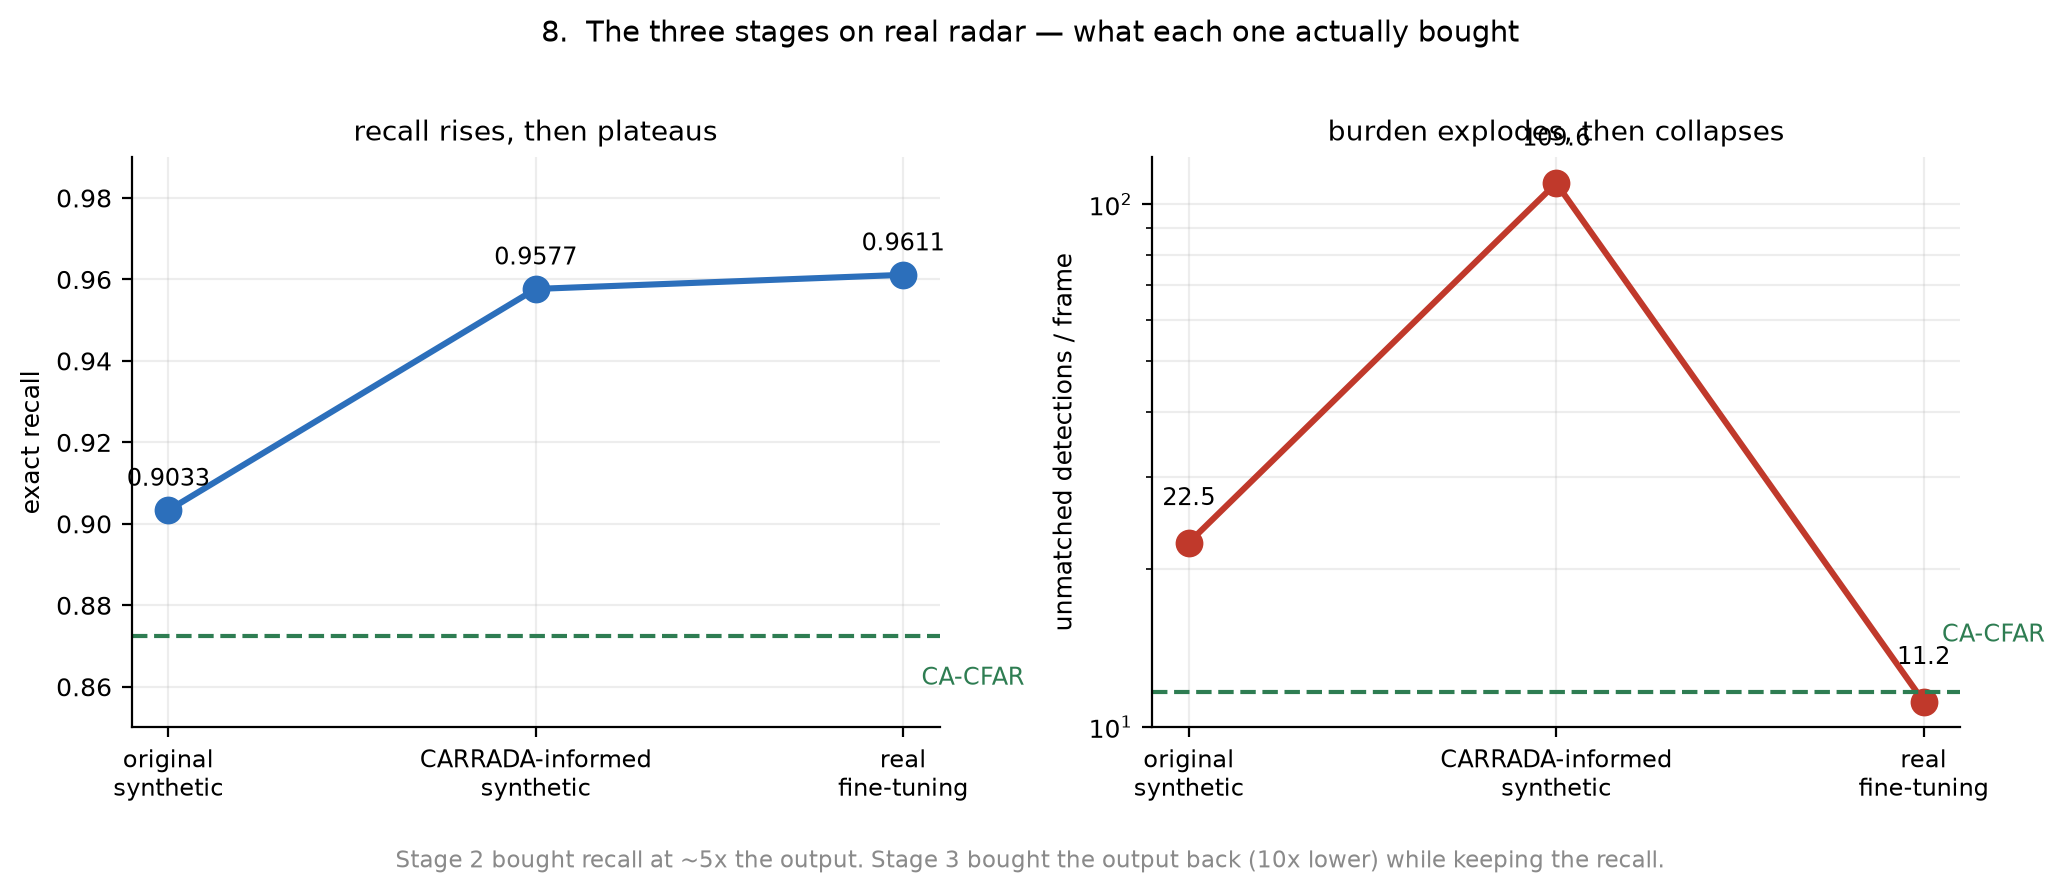
\includegraphics[width=0.96\textwidth]{figures/Chapter8/ch8_fig1_progression.png}
\caption[The three training domains on real radar]{The three training domains, both scored on the
CARRADA validation split so the four arms are directly comparable. \textbf{Left}: exact dense-mask
recall rises with domain alignment and then plateaus --- real supervision adds no established recall
over target-informed synthetic training. \textbf{Right}: output burden, on a logarithmic axis,
explodes under target-informed synthetic training and collapses under real fine-tuning. The
classical baseline is the dashed line in both panels. Recall alone would have told less than half
of this story.}
\label{fig:progression}
\end{figure}

\begin{figure}[H]
\centering
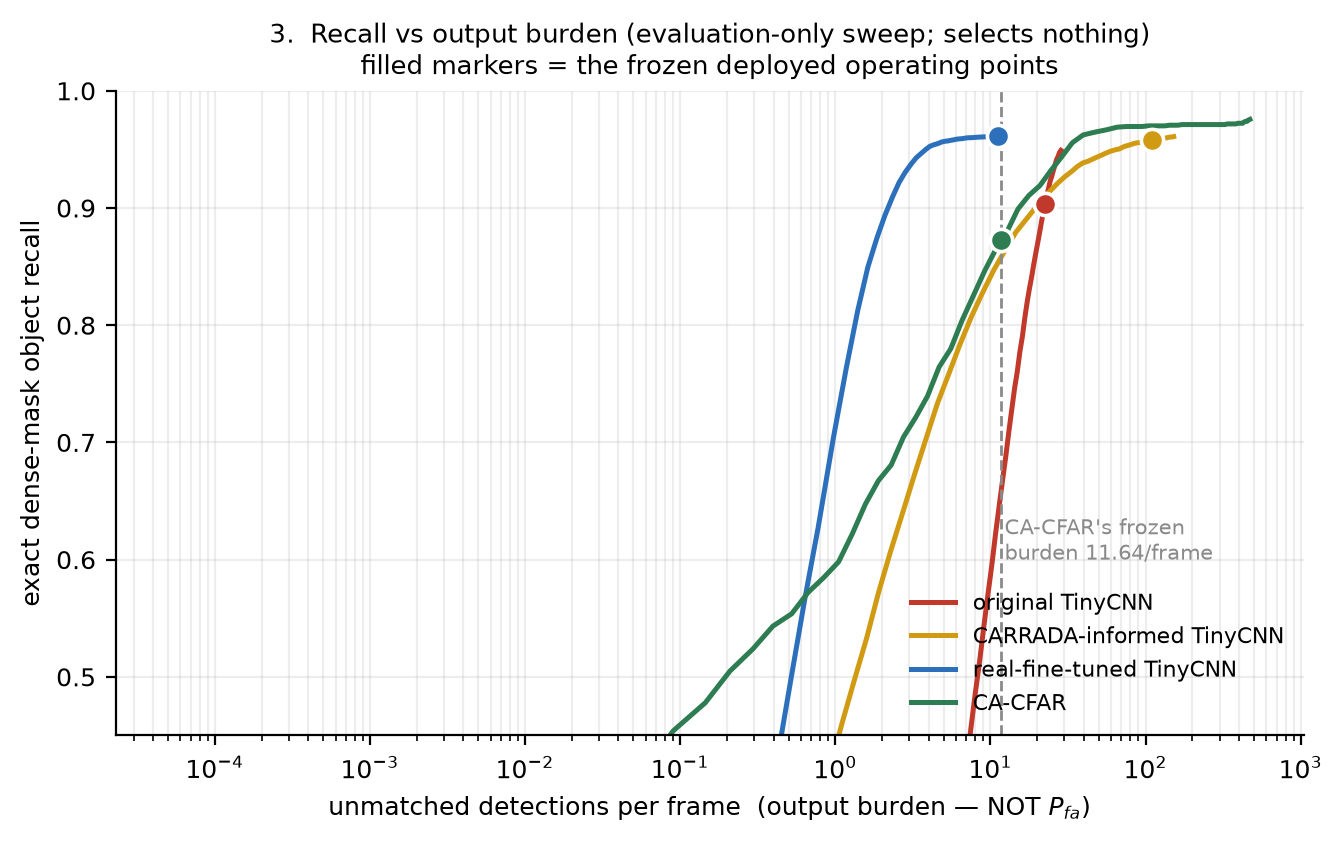
\includegraphics[width=0.92\textwidth]{figures/Chapter8/ch8_fig2_burden_curve.png}
\caption[Recall against output burden on the validation split]{Recall against output burden on the
CARRADA validation split, from an evaluation-only threshold sweep that selected nothing; filled
markers are the frozen deployed operating points. The fine-tuned detector reaches its recall
ceiling at an output density where the classical detector is still well short of it, and its entire
candidate list ends near \FtValBurdenFt{} detections per frame --- it cannot be pushed to the
densities the other learned arms occupy. \textbf{Unmatched detections are an output-burden measure,
not a false-alarm rate}: CARRADA annotates the objects that were labelled, not every scatterer
present.}
\label{fig:burdencurve}
\end{figure}

\section{Conclusion}
\label{sec:domaingapconclusion}

Two follow-up experiments, each answering the question the previous stage left open.

Target-domain-informed synthetic training showed that the synthetic training distribution was a
material part of the transfer failure: recalibrating the background toward measured target-domain
statistics recovered a large part of the lost real-data recall \emph{without any real frame entering
neural optimisation}. It also showed that recall is not a sufficient summary, because the recovery
came with roughly \CiTestBurdenRatio{} times the output density and did not survive burden matching
against the classical baseline.

Real-domain fine-tuning then produced the strongest learned-versus-classical result in this thesis:
higher exact recall than CA-CFAR at a slightly lower output burden, on sequences no detector in this
project had previously scored. Its contribution was not recall --- that had already been recovered
--- but selectivity, cutting output by about an order of magnitude while holding recall.

Taken together these two stages convert Chapter~\ref{chp:realdata}'s negative result into a
conditional one. The learned detector's advantage was never a fixed property of the architecture. It
was a property of how well its training distribution matched deployment, and it became a genuine
advantage over the classical baseline only once the deployment domain was represented during
training --- first statistically, then with real supervision.
